\subsection{Typen von Abbildungen}
Seinen A und B zwei Mengen und $f:{A}\longrightarrow{B}$ eine Abbildungsvorschrift.
Dann gibt es 3 besondere Typen von Abbildungen:

\begin{description}
\item[surjektive Abbildung] \emph{alle} Elemente von B mindestens einmal erfassen
\item[injektive Abbildungen] alle Elemente von A erhalten \emph{unterschiedliche} Elemente aus B
\item[bijektive Abbildungen] \emph{surjektiv und injektiv} zu gleich: alle A erhalten genau ein B und alle B werden getroffen.
Dies impliziert die Umkehrbarkeit der Funktion. Eine Sonderform der bijektiven
Abbildung ist die \emph{Identität}. Dabei wird jedes Element sich selbst zugeordnet.
\end{description}

\begin{figure}
\subfigure[surjektive
Abbildung]{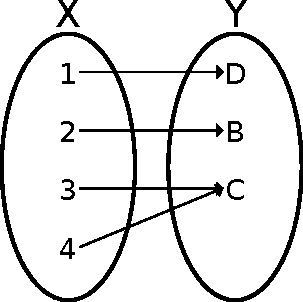
\includegraphics[width=3cm]{Surjection.pdf}}\hfill
\subfigure[injektive
Abbildung]{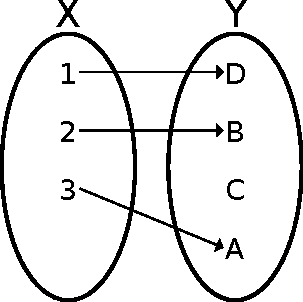
\includegraphics[width=3cm]{Injection.pdf}}\hfill
\subfigure[bijektive
Abbildungen]{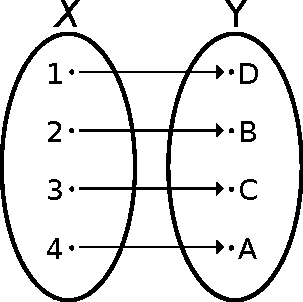
\includegraphics[width=3cm]{Bijection.pdf}}\hfill
\subfigure[identische
Abbildungen]{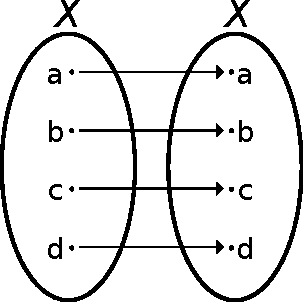
\includegraphics[width=3cm]{Identitaet.pdf}}
\end{figure}